\documentclass[a4paper]{article}
\usepackage{ctex}
\usepackage[affil-it]{authblk}
\usepackage[backend=bibtex,style=numeric]{biblatex}
\usepackage{amsmath,amsthm,amssymb,amsfonts}
\usepackage{graphicx}
\usepackage{bm}

\usepackage{geometry}
\geometry{margin=1.5cm, vmargin={0pt,1cm}}
\setlength{\topmargin}{-1cm}
\setlength{\paperheight}{29.7cm}
\setlength{\textheight}{25.3cm}

\addbibresource{citation.bib}

\begin{document}
% =================================================
\title{微分方程数值解 2026 春夏作业二}

\author{曾申昊 3220100701
  \thanks{邮箱: \texttt{3097714673@qq.com}
                            \texttt{或} \texttt{3220100701@zju.edu.cn}}}
\affil{浙江大学}

\date{更新时间: \today}

\maketitle

% ============================================
\section*{Exercise 11.6}

\par 将不等式左边具体写出：
\begin{equation}
    \begin{gathered}
        \frac{1}{\lVert A\rVert_2\lVert A^{-1}\rVert_2}
        \frac{\lVert A\bm{e}\rVert_2}{\lVert A\bm{x}\rVert_2}
        \leq \frac{\lVert \bm{e}\rVert_2}{\lVert \bm{x}\rVert_2}\\
        \frac{\lVert A\bm{e}\rVert_2}{\lVert A^{-1}\rVert_2\lVert A\bm{x}\rVert_2}
        \leq \frac{\lVert A\rVert_2\lVert \bm{e}\rVert_2}{\lVert \bm{x}\rVert_2}
    \end{gathered}
\end{equation}
\par 由 $\lVert A\bm{e}\rVert_2\leq \lVert A\rVert_2\lVert \bm{e}\rVert_2$
和 $\lVert A^{-1}\rVert_2\lVert A\bm{x}\rVert_2\geq \lVert \bm{x}\rVert_2$ 可得不等式左边成立。
类似的有：
\begin{equation}
    \begin{gathered}
        \frac{\lVert \bm{e}\rVert_2}{\lVert \bm{x}\rVert_2}
        \leq
        \lVert A\rVert_2\lVert A^{-1}\rVert_2
        \frac{\lVert A\bm{e}\rVert_2}{\lVert A\bm{x}\rVert_2}\\
        \frac{\lVert \bm{e}\rVert_2}{\lVert A\rVert_2\lVert \bm{x}\rVert_2}
        \leq
        \frac{\lVert A^{-1}\rVert_2\lVert A\bm{e}\rVert_2}{\lVert A\bm{x}\rVert_2}
    \end{gathered}
\end{equation}
\par 由 $\lVert \bm{e}\rVert_2\leq \lVert A^{-1}\rVert_2\lVert A\bm{e}\rVert_2$
和 $\lVert A\rVert_2\lVert \bm{x}\rVert_2\geq \lVert A\bm{x}\rVert_2$ 可得不等式右边成立。

\section*{Exercise 11.11}

\par 如图 \ref{fig:Exercise11-11} 所示， $k_{\text{max}}=
\dfrac{2}{L_{\text{min}}}=
\dfrac{2}{\frac{1}{3}}=6$，
也就是 $\dfrac{1}{h}=6$。

\begin{figure}[ht]
    \centering
    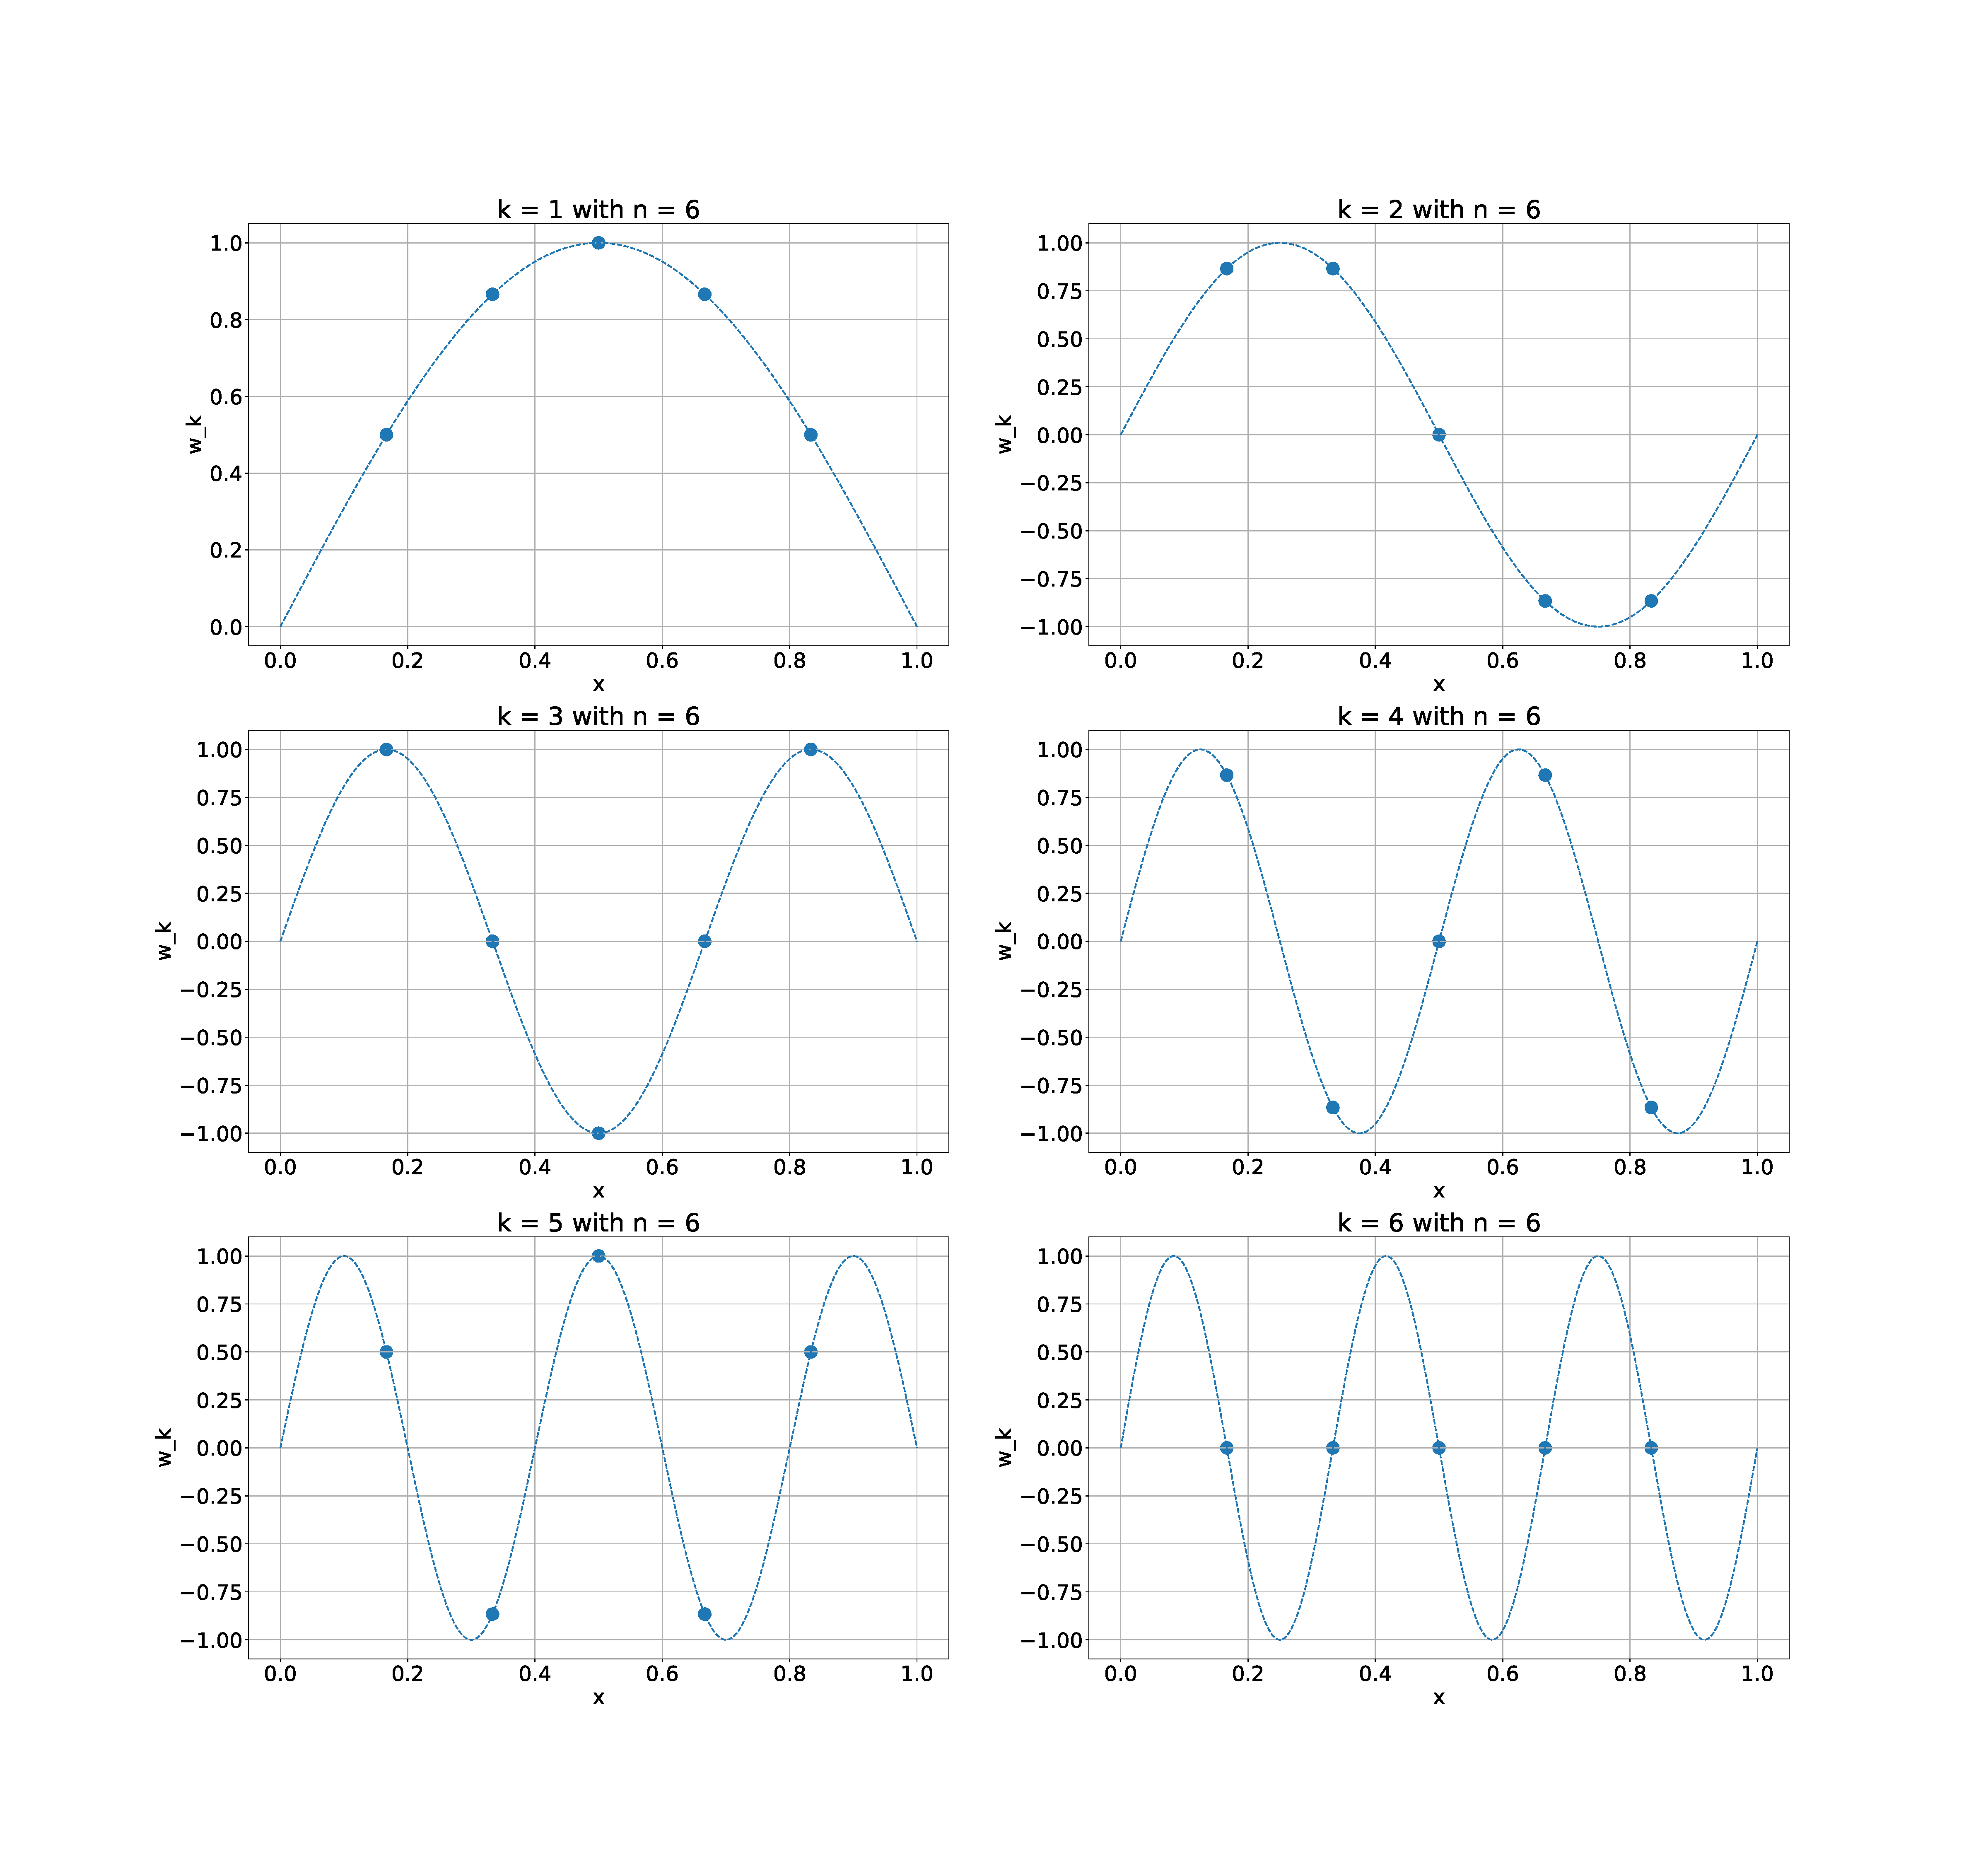
\includegraphics[width=0.9\textwidth]{figure/Exercise11-11.pdf}
    \vspace*{-2em}
    \caption{Exercise 11.11}
    \label{fig:Exercise11-11}
\end{figure}

\section*{Exercise 11.14}

\begin{figure}[ht]
    \centering
    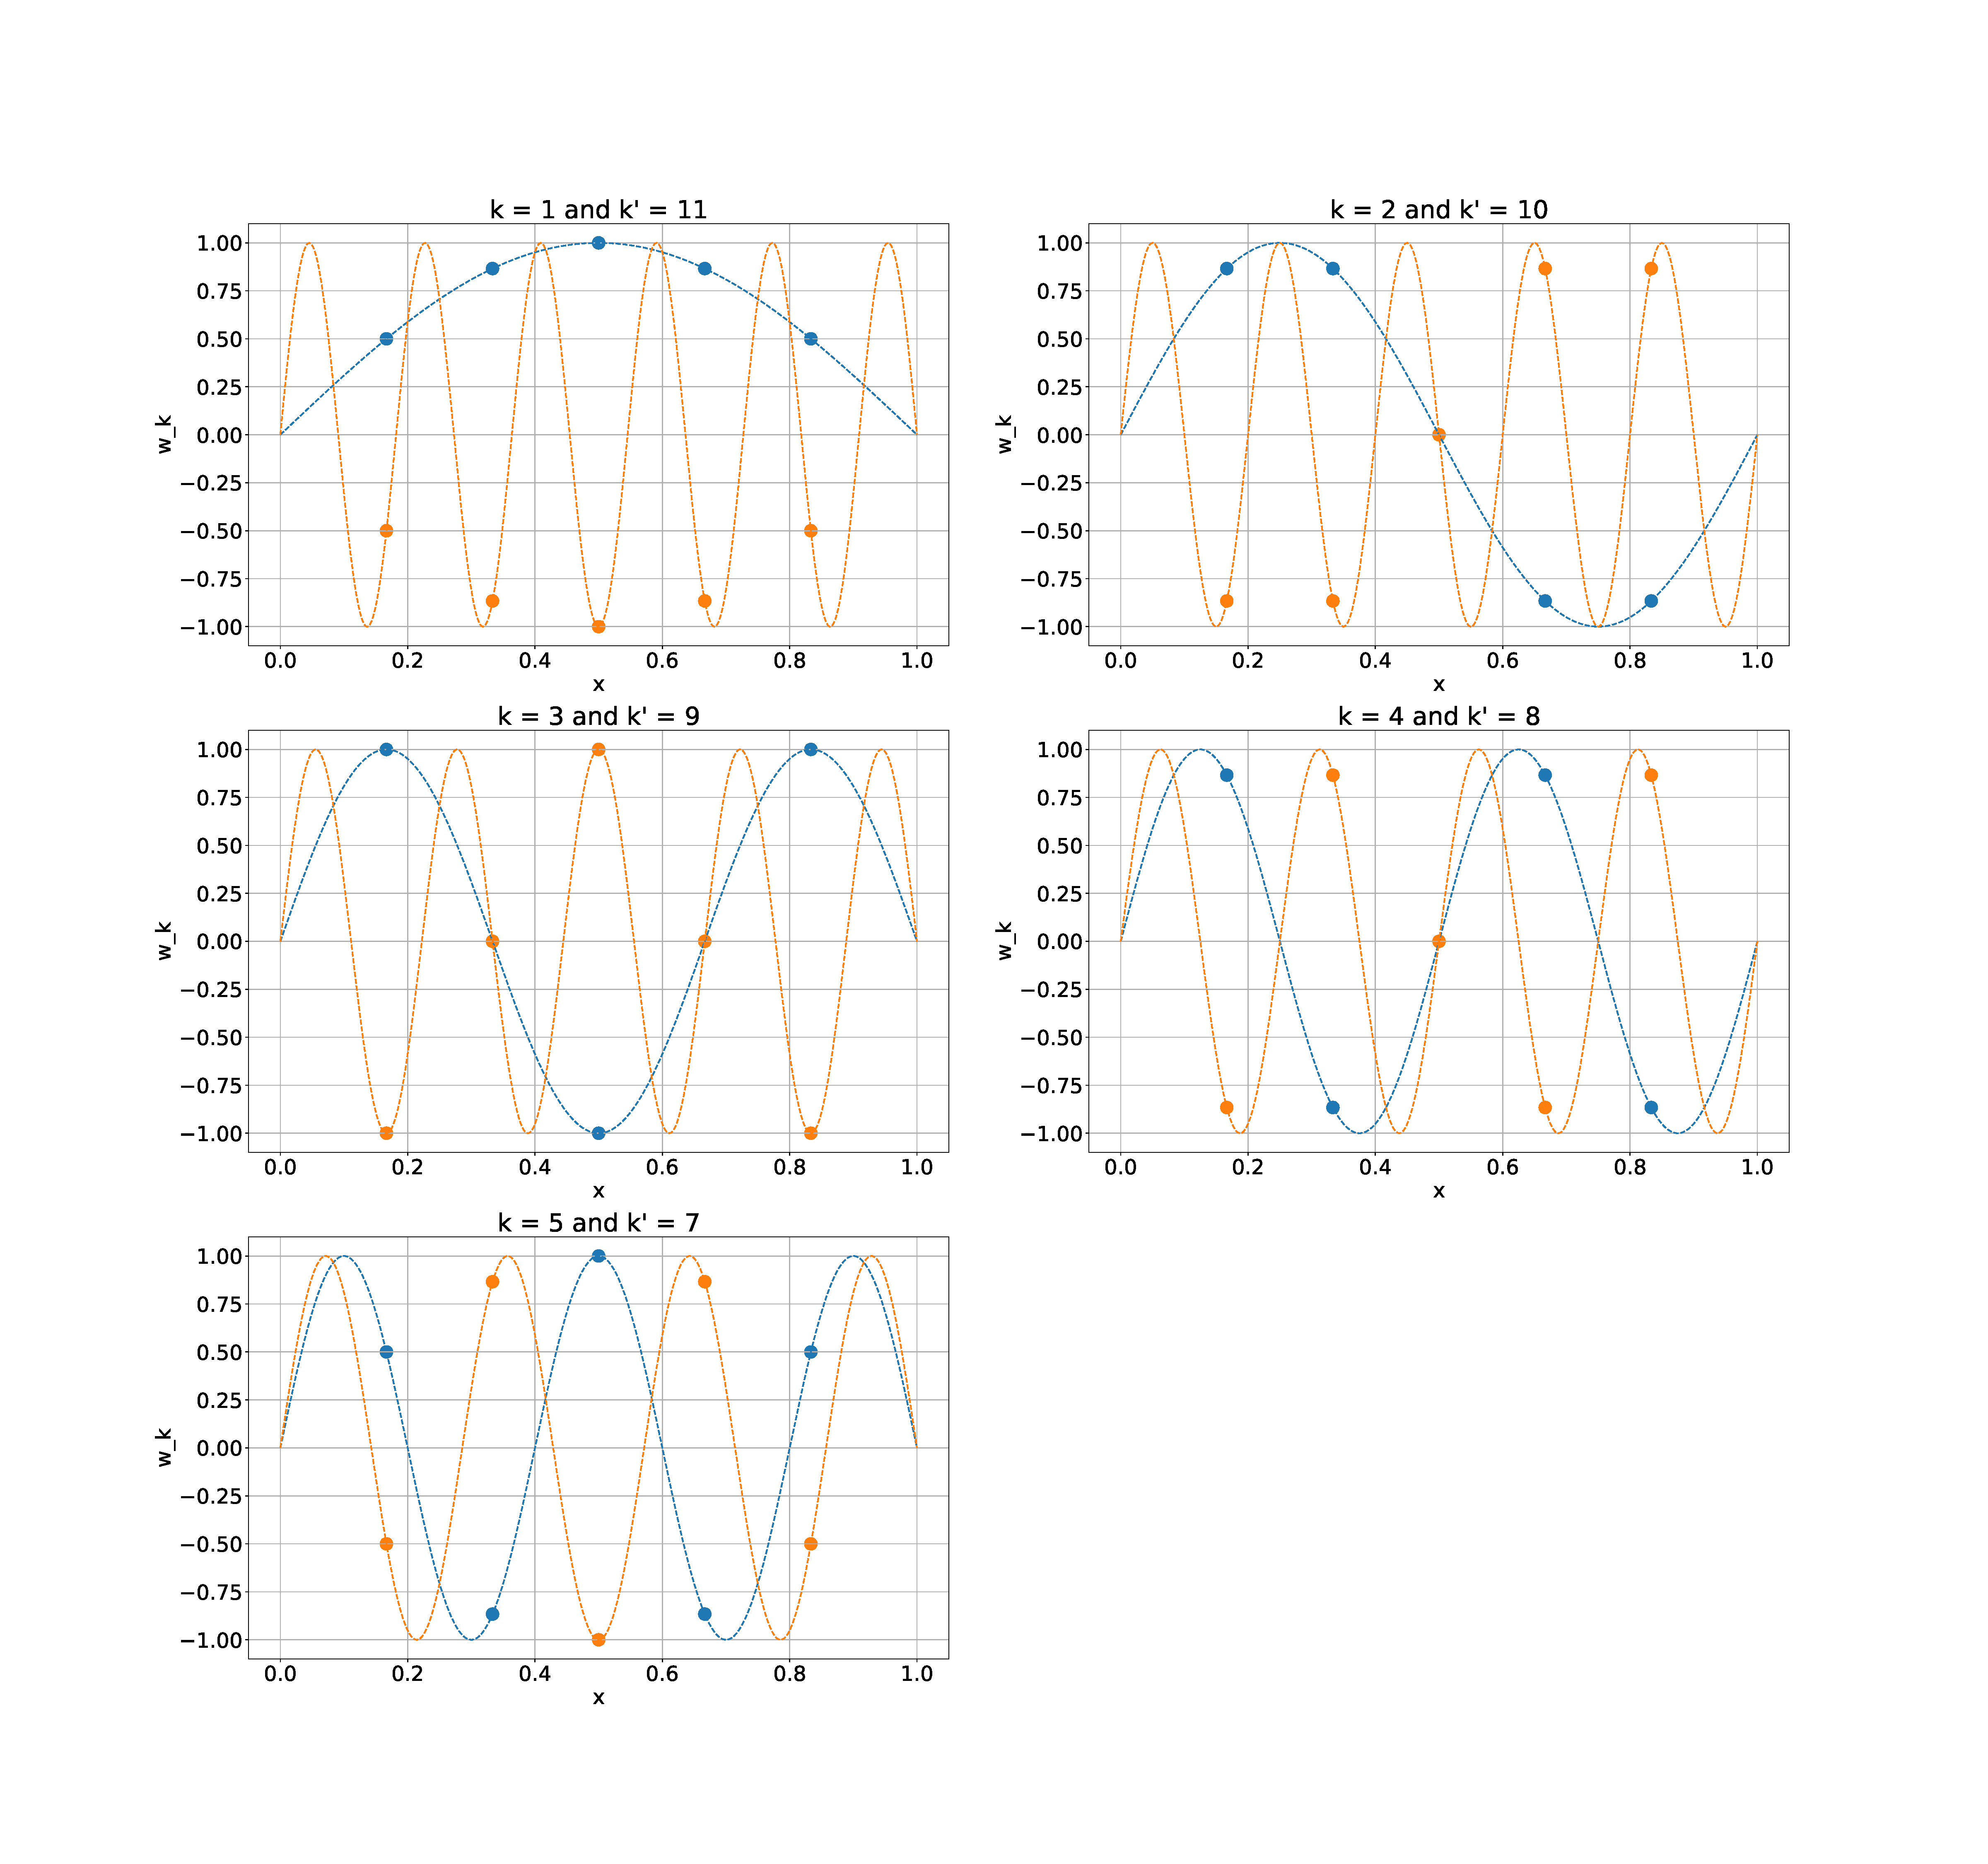
\includegraphics[width=0.9\textwidth]{figure/Exercise11-14.pdf}
    \vspace*{-2em}
    \caption{Exercise 11.14}
    \label{fig:Exercise11-14}
\end{figure}
\par 对于 $n=6$ 计算得到 $\bm{w}_k$ 的值
并绘制图像如图 \ref{fig:Exercise11-14} 所示，
可以看到低频和高频的散点图像恰好为相反数。

\section*{Exercise 11.17}

\par 加权 Jacobi 迭代的迭代矩阵为
\begin{equation}
    \begin{aligned}
        T_{\omega}
        &=(1-\omega)I+\omega D^{-1}(L+U)\\
        &=(1-\omega)I+\omega D^{-1}(D-A)\\
        &=I-\omega D^{-1}A\\
        &=I-\frac{\omega h^2}{2} A\\
    \end{aligned}
\end{equation}
\par 考虑矩阵 $A$ 的特征向量 $\bm{w}_k$ 以及对应的特征值 
$\lambda_k = \dfrac{4}{h^2}\sin^2\dfrac{k\pi}{2n}$，其中 $k=1,2,\cdots,n-1$。
代入得到：
\begin{equation}
    \begin{aligned}
        T_{\omega}\bm{w}_k
        &=\left(I-\frac{\omega h^2}{2} A\right)\bm{w}_k\\
        &=\left(1-\frac{\omega h^2}{2}\lambda_k\right)\bm{w}_k\\
        &=\left(1-2\omega\sin^2\dfrac{k\pi}{2n}\right)\bm{w}_k
    \end{aligned}
\end{equation}
\par 因此 $\bm{w}_k$ 也是 $T_{\omega}$ 的特征向量，
并且对应的特征值为 $\lambda_k(T_{\omega}) = 1-2\omega\sin^2\dfrac{k\pi}{2n}$。

\section*{Exercise 11.18}

\begin{figure}[ht]
    \centering
    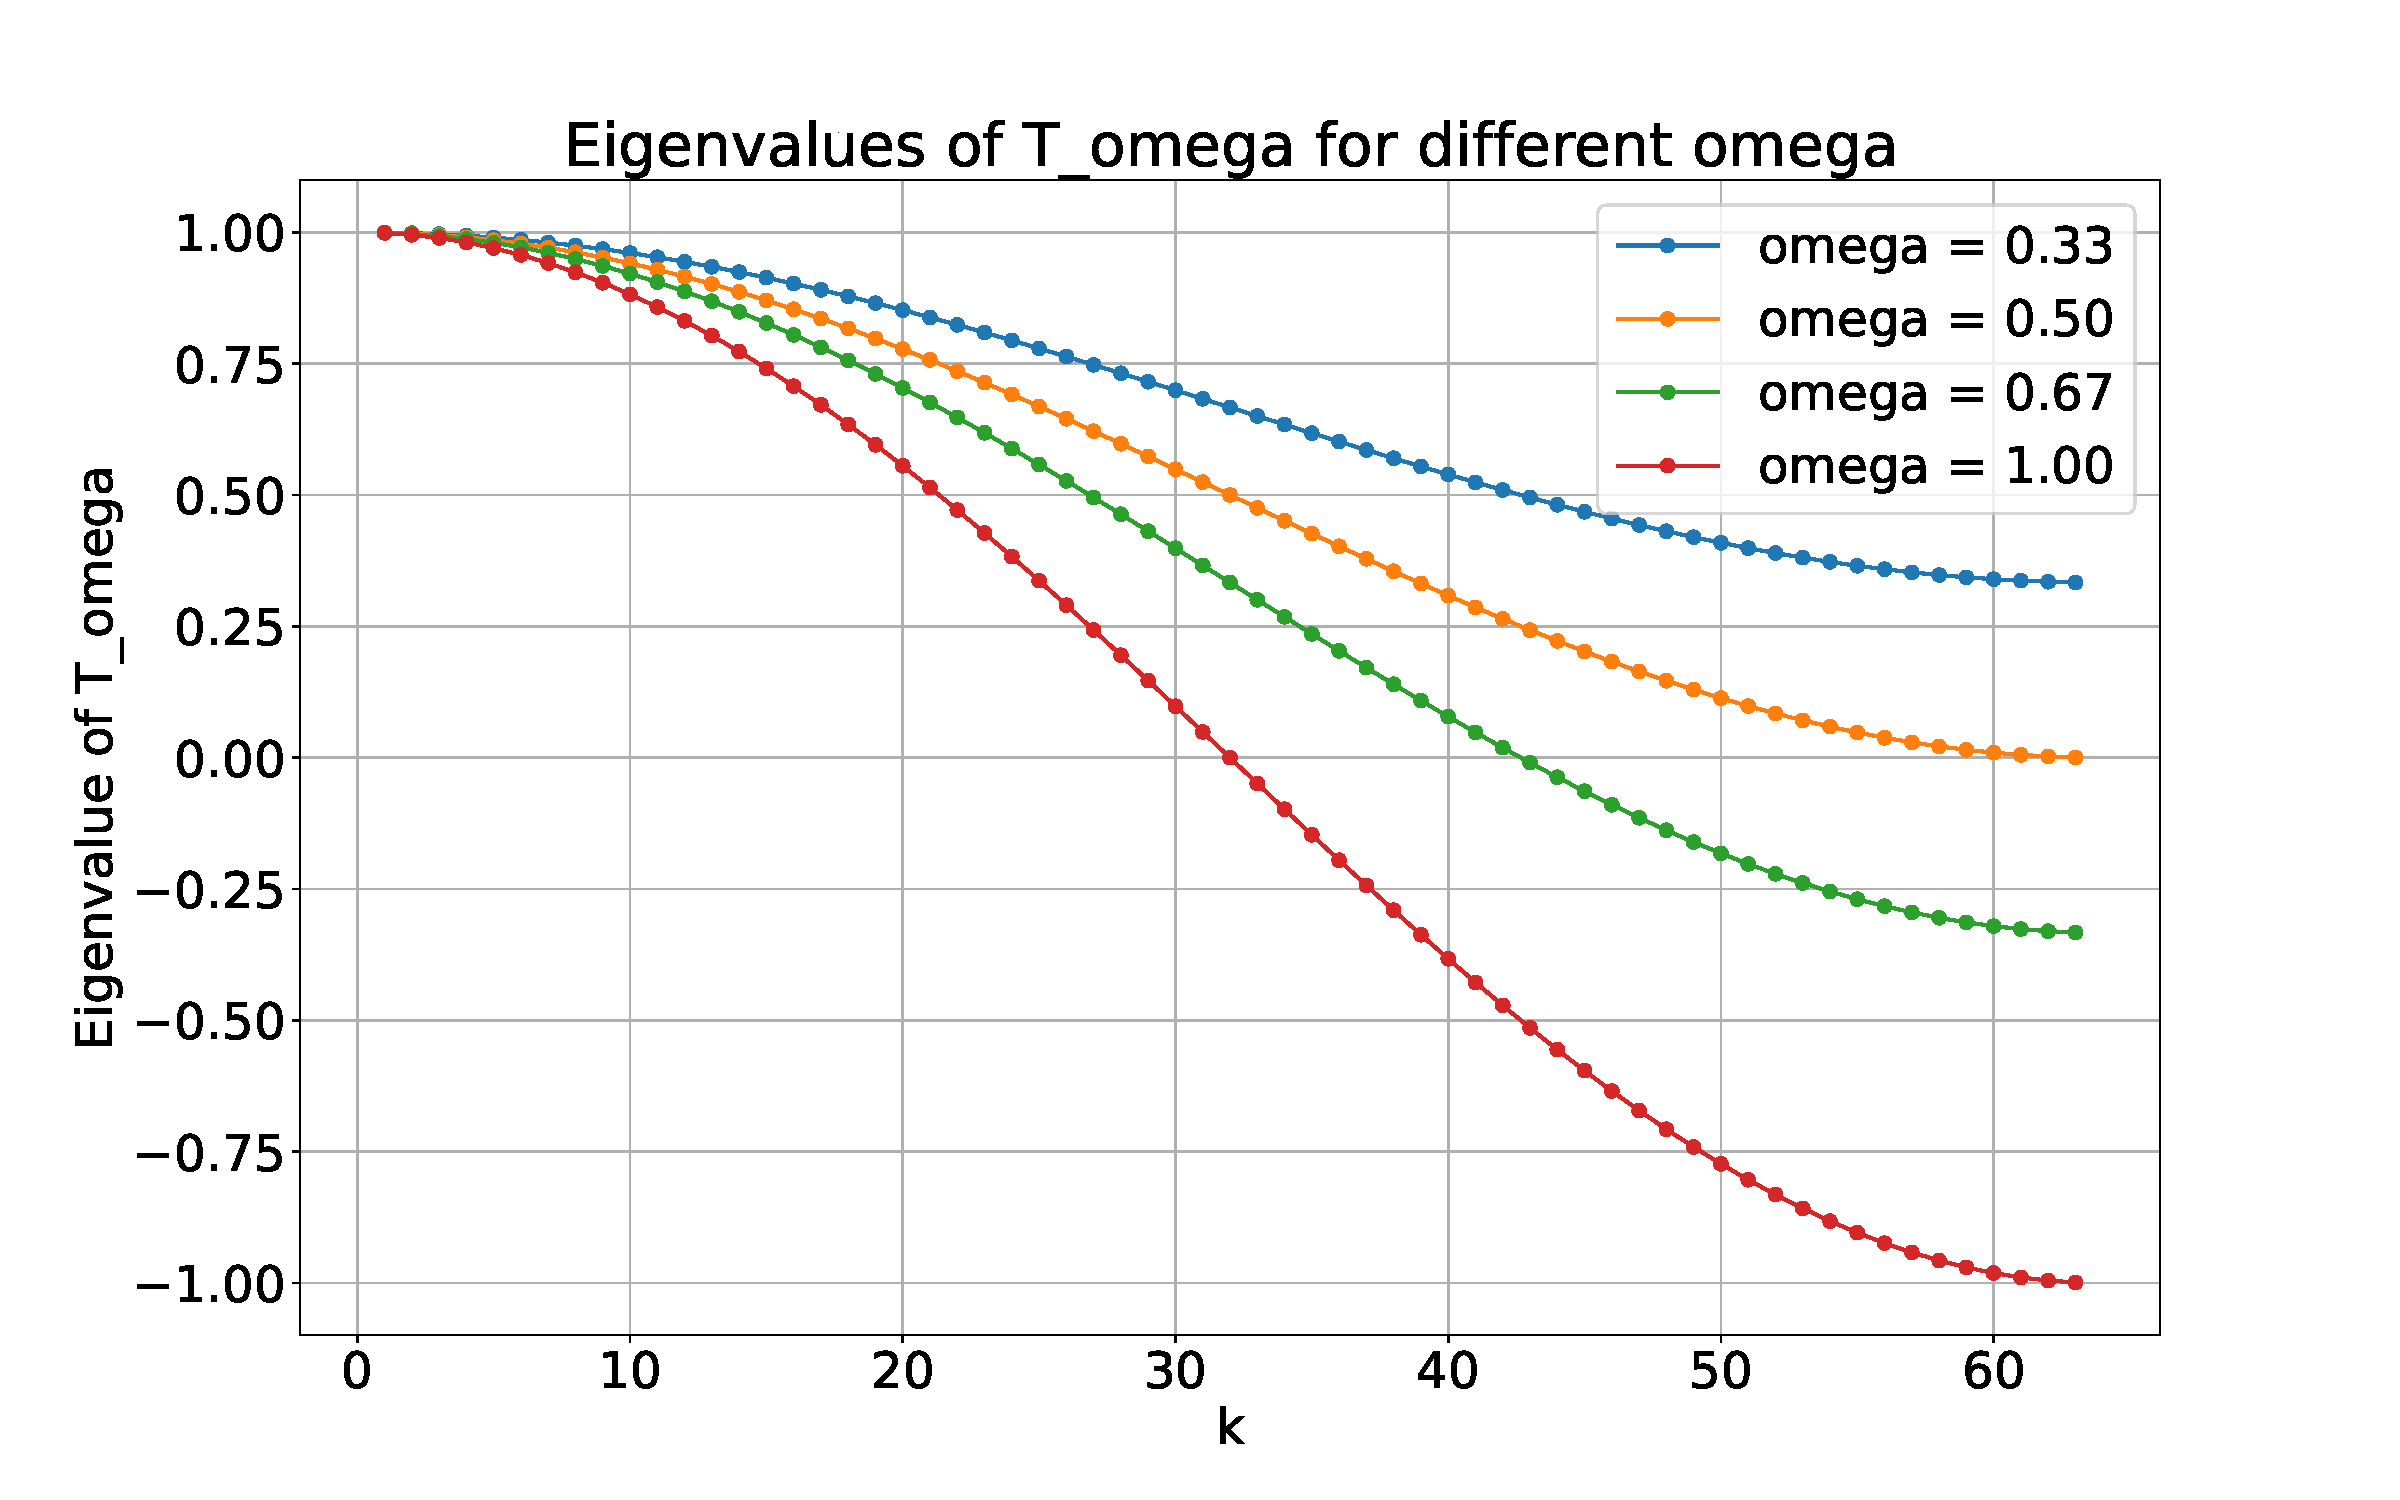
\includegraphics[width=0.65\textwidth]{figure/Exercise11-18.pdf}
    \caption{Exercise 11.18}
    \label{fig:Exercise11-18}
\end{figure}

\par 对于 $n=64$和  $\forall\omega\in[0,1]$ 有：
\begin{equation}
    \rho(T_{\omega})
    \geq \left|1-2\sin^2\dfrac{63 \pi}{128}\right|
    \approx 0.9986
\end{equation}

\section*{Exercise 11.21}

\begin{figure}[ht]
    \centering
    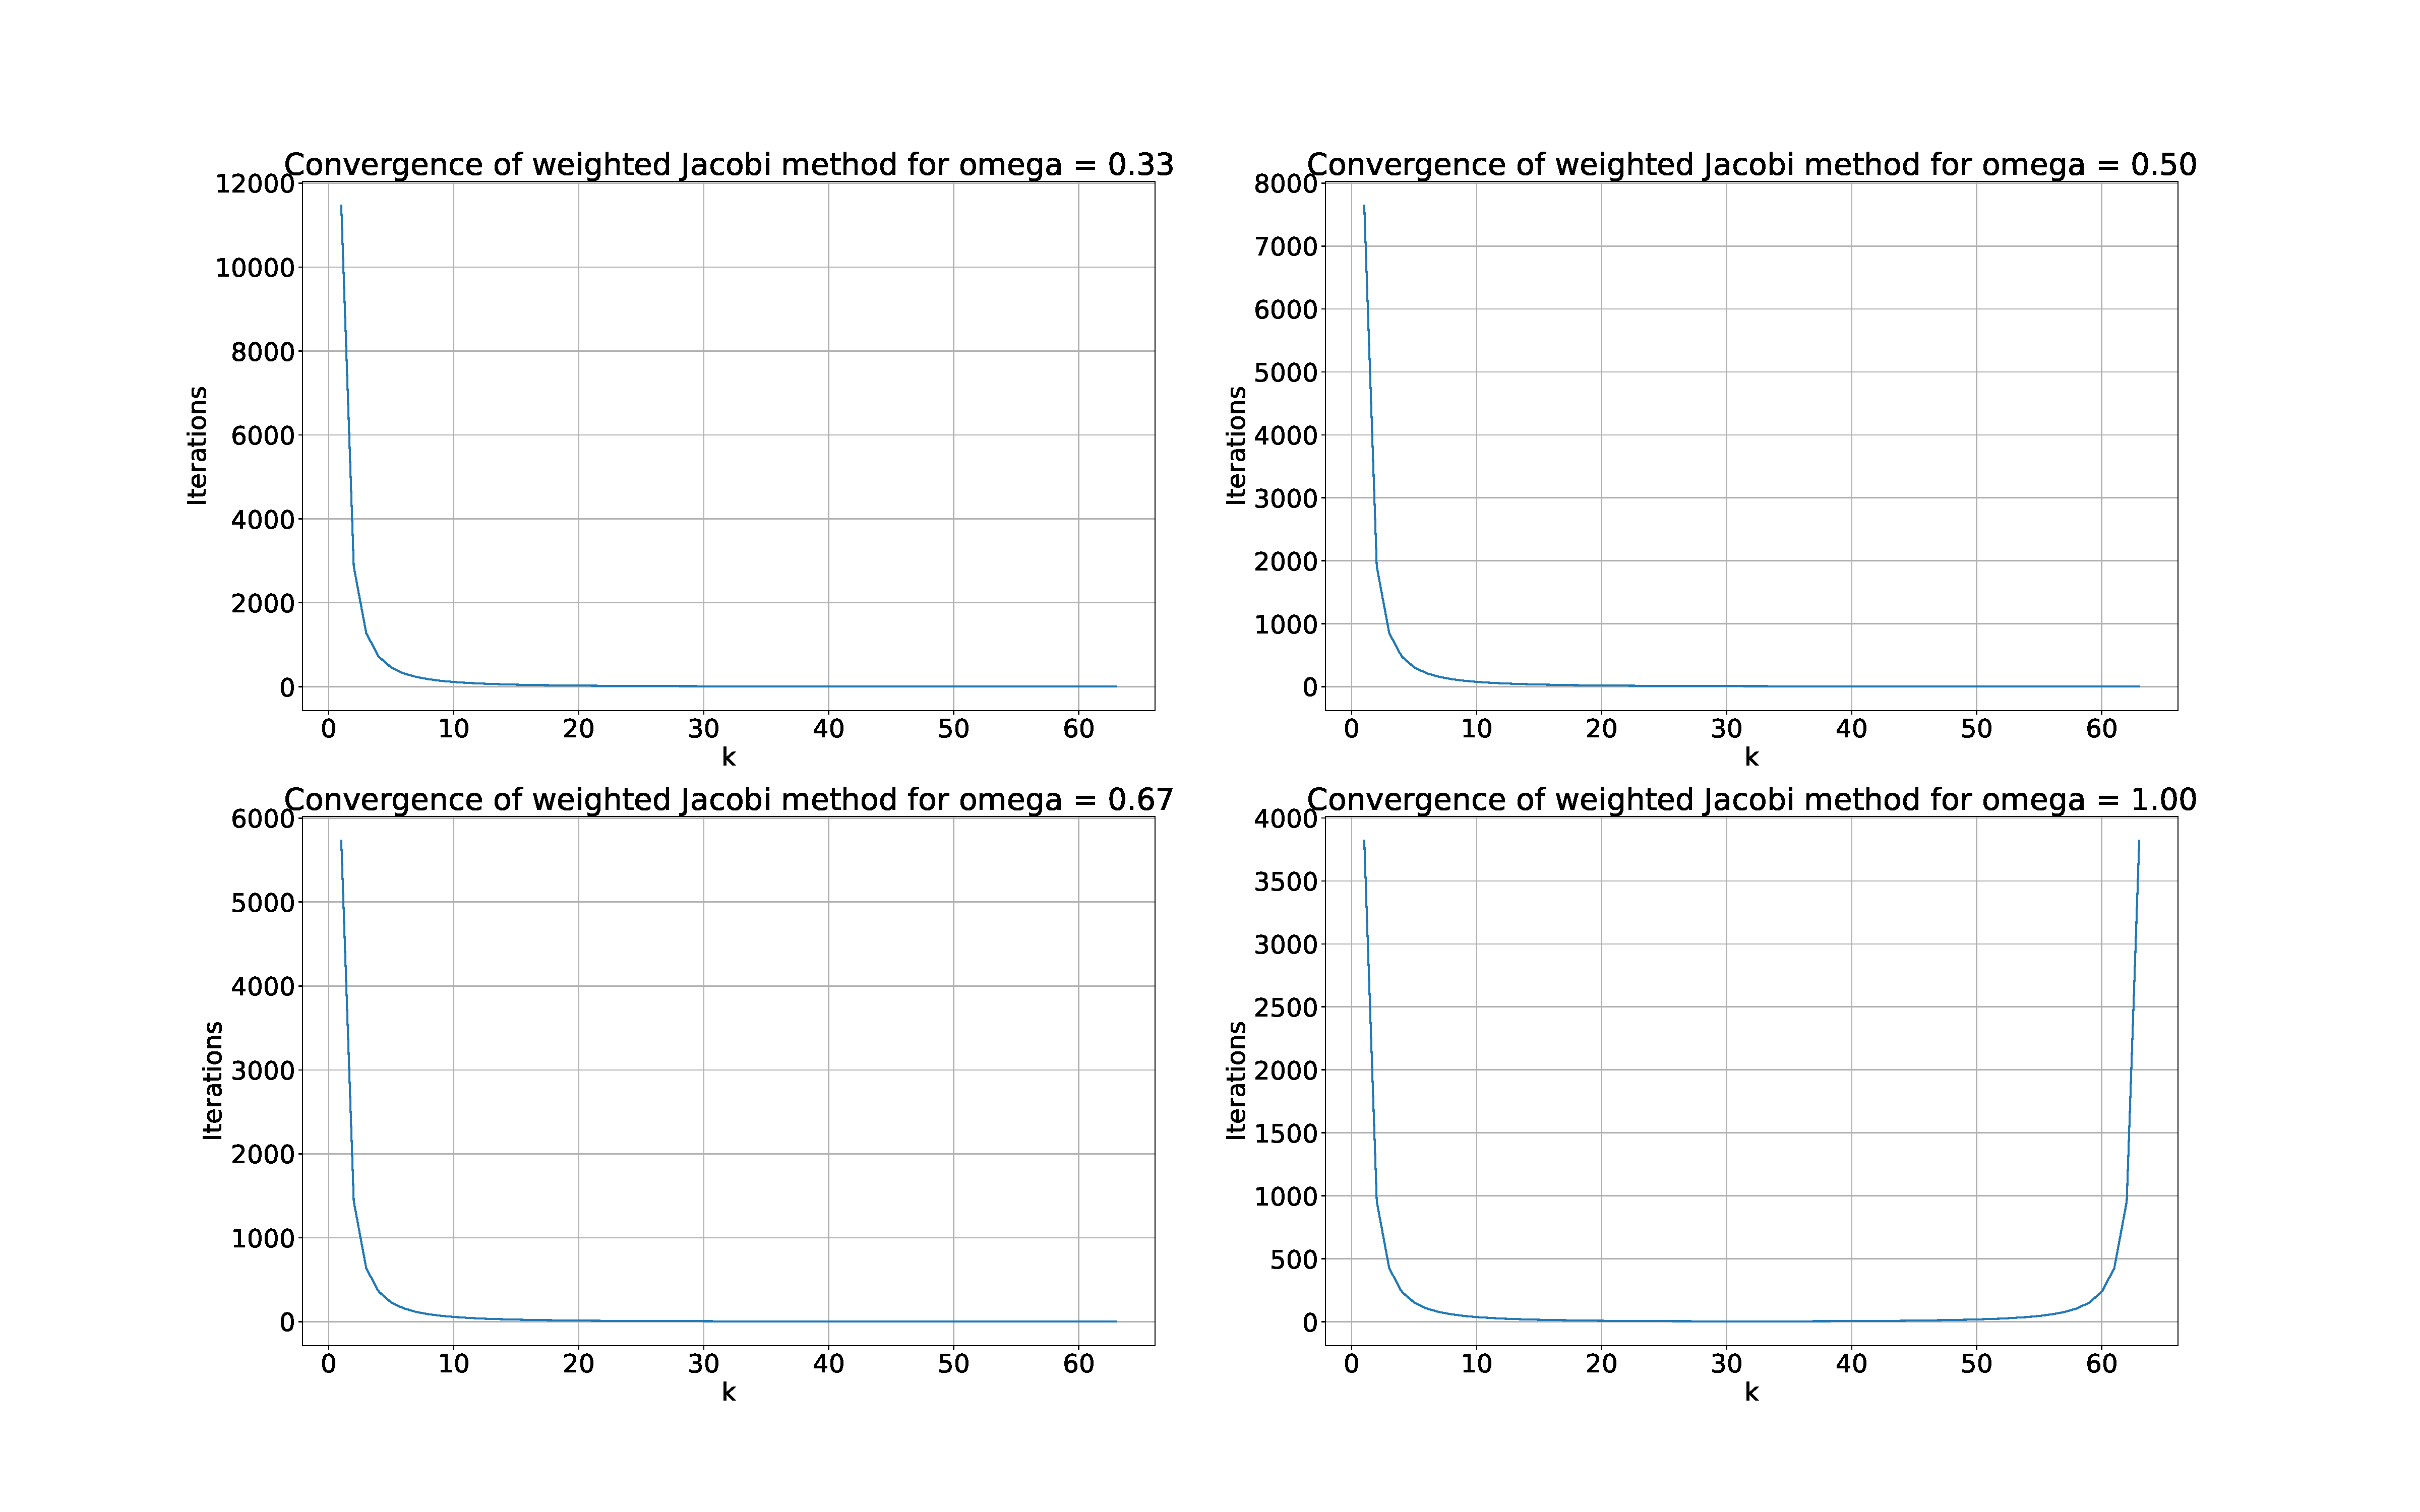
\includegraphics[width=0.9\textwidth]{figure/Exercise11-21.pdf}
    \vspace*{-2em}
    \caption{Exercise 11.21}
    \label{fig:Exercise11-21}
\end{figure}
\par 如图 \ref{fig:Exercise11-21} 所示，
可以得到与讲义中一致的结论：对于 $\omega=1$，高频分量难以衰减；
对于 $\omega=0.67$则不会出现这种情况。

\section*{Exercise 11.35}

\begin{equation}
    \begin{aligned}
        &\quad2\left(\text{WU}\cdot2^{-(m-1)\text{D}}\right)\left(1+2^{-\text{D}}\right)
        +2\left(\text{WU}\cdot2^{-(m-2)\text{D}}\right)\left(1+2^{-\text{D}}+2^{-2\text{D}}\right)
        +\cdots
        +2\left(\text{WU}\cdot2^{0}\right)\left(1+2^{-\text{D}}+\cdots+2^{-m\text{D}}\right)\\
        &\leq2\text{WU}\left(1+2\cdot2^{-\text{D}}+3\cdot2^{-2\text{D}}
        +\cdots+m\cdot2^{-(m-1)\text{D}}+(m+1)\cdot2^{-m\text{D}}\right)\\
        &\leq\frac{2}{\left(1-2^{\text{D}}\right)^2}\text{WU}
    \end{aligned}
\end{equation}
\par 最后一步是由 $\displaystyle\sum_{m=0}^{\infty} x^m=\dfrac{1}{1-x}$ 两边求导得到的:
\begin{equation}
    \displaystyle\sum_{m=1}^{\infty} mx^{m-1}=\dfrac{1}{(1-x)^2}
\end{equation}
\par 对于 $D=1,2,3$，计算量上界分别为
\begin{equation}
    \left\{
        \begin{aligned}
            &D=1:\quad\frac{2}{(1-2^{-1})^2}\text{WU} = 8\text{WU}\\
            &D=2:\quad\frac{2}{(1-2^{-2})^2}\text{WU} = \frac{32}{9}\text{WU}\\
            &D=3:\quad\frac{2}{(1-2^{-3})^2}\text{WU} = \frac{128}{49}\text{WU}
        \end{aligned}
    \right.
\end{equation}

\section*{Exercise 11.41}

\begin{figure}[ht]
    \centering
    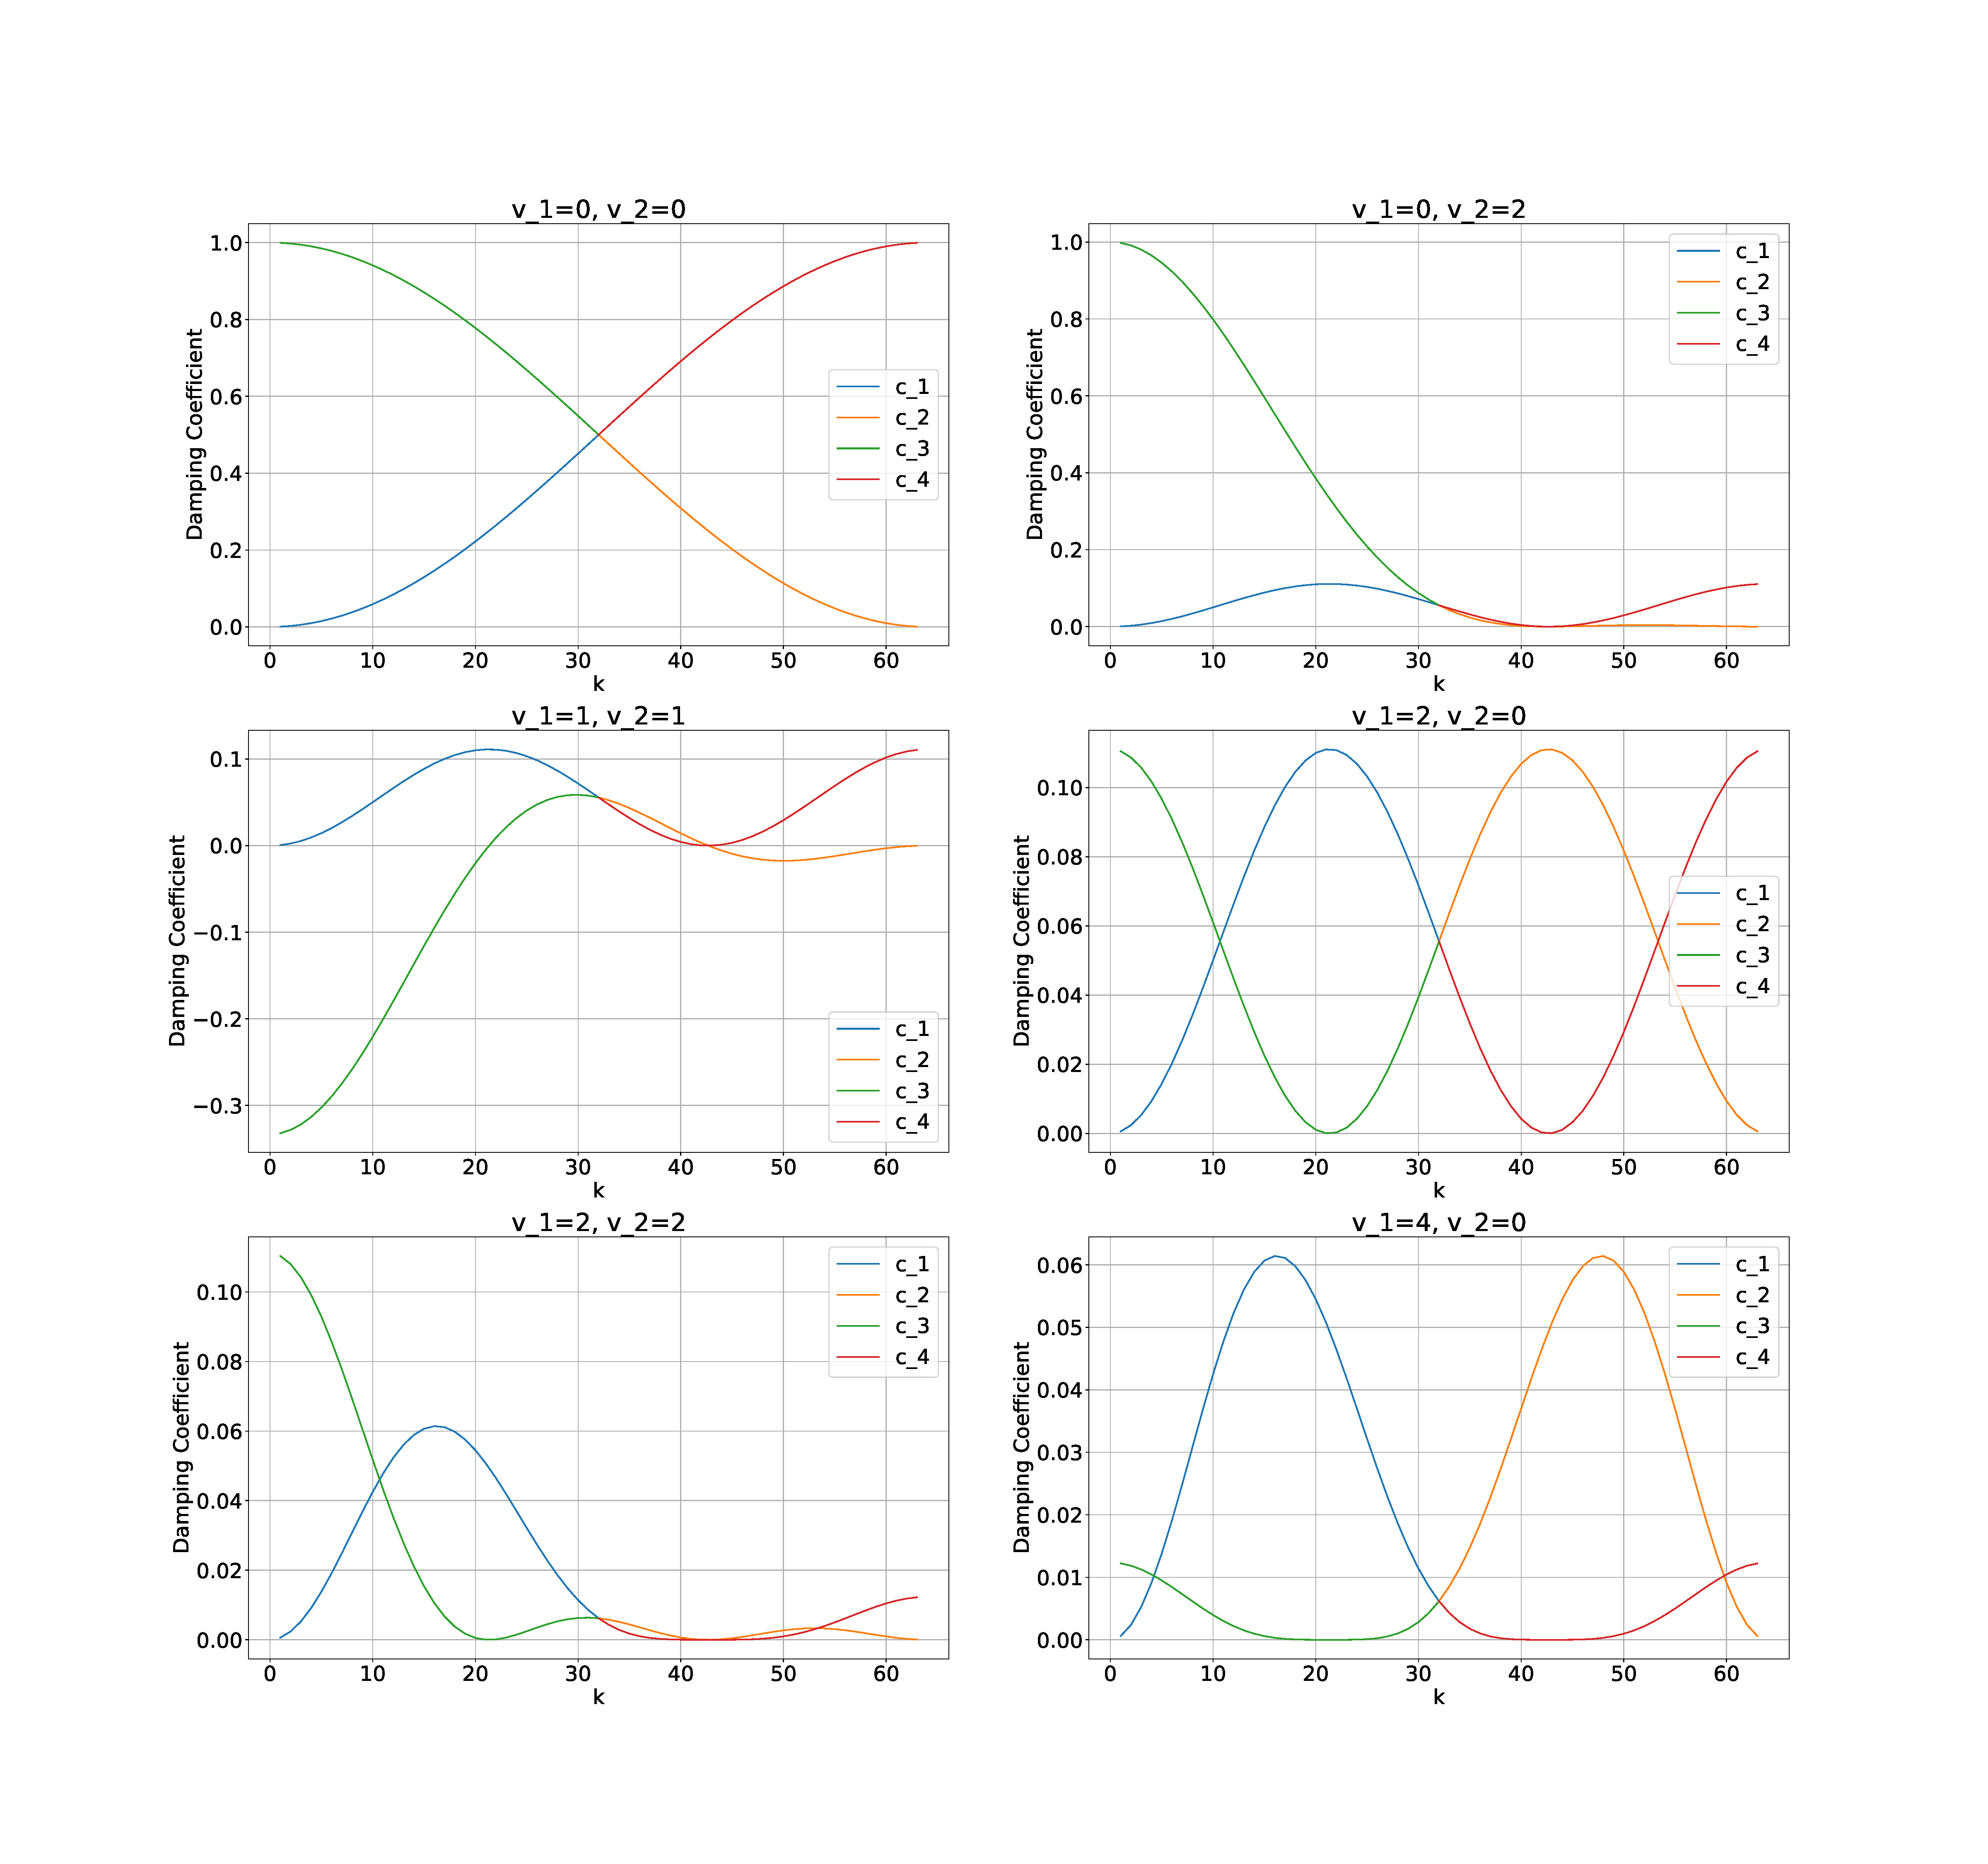
\includegraphics[width=0.9\textwidth]{figure/Exercise11-41.pdf}
    \vspace*{-2em}
    \caption{Exercise 11.41 $n=64$}
    \label{fig:Exercise11-41}
\end{figure}
\par 为了估计$\rho(\text{TG})$，
需要计算 $\lambda_k(\text{TG})$ 的值：
\begin{equation}
    \begin{gathered}
        (c_1-\lambda)(c_4-\lambda)-c_2c_3=0\\
        \lambda^2-(c_1+c_4)\lambda+c_1c_4-c_2c_3=0\\
        \lambda=\frac{(c_1+c_4)\pm\sqrt{(c_1+c_4)^2-4(c_1c_4-c_2c_3)}}{2}  
    \end{gathered}
\end{equation}
\par 将具体分量代入：
\begin{equation}
    \left\{
        \begin{aligned}
            &c_1 = \lambda_k^{v_1+v_2}s_k\\
            &c_2 = \lambda_k^{v_1}\lambda_{k'}^{v_2}s_k\\
            &c_3 = \lambda_{k'}^{v_1}\lambda_k^{v_2}c_k\\
            &c_4 = \lambda_{k'}^{v_1+v_2}c_k
        \end{aligned}
    \right.
\end{equation}
\par 可以得到：
\begin{equation}
    \left\{
        \begin{aligned}
            &\lambda_1 = c_1+c_4\\
            &\lambda_2 = 0
        \end{aligned}
    \right.
\end{equation}
\par 从图 \ref{fig:Exercise11-41} 可以看到对于 $v_1=0$和$v_2=0$，
$\rho(\text{TG})=\lambda_1=1$；对于其他情况 $\rho(\text{TG})=\lambda_1 \lessapprox  0.1$。

\section*{Exercise 11.45}

\par Full Weight 算子 $I_{h}^{2h}:\mathbb{R}^{\frac{n}{2}} \to \mathbb{R}^{n-1}$
具体分量为：
\begin{equation}
    I_{h}^{2h}=\frac{1}{4}
    \begin{bmatrix}
        1 & 2 & 1 & 0 & \cdots & 0 & 0 & 0 & 0\\
        0 & 1 & 2 & 1 & \cdots & 0 & 0 & 0 & 0\\
        \vdots & \vdots & \vdots & \vdots & \ddots & \vdots& \vdots& \vdots& \vdots\\
        0 & 0 & 0 & 0 & \cdots & 1 & 2 & 1 & 0\\
        0 & 0 & 0 & 0 & \cdots & 0 & 1 & 2 & 1
    \end{bmatrix}
\end{equation}
\par 根据线性代数知识以及 \textbf{Lemma 11.43}，有 
\begin{equation}
    \mathcal{R}(I_{h}^{2h}) = \mathcal{N}\left((I_{h}^{2h})^T\right)^{\perp}
    =\mathcal{N}\left(I_{2h}^{h}\right)^{\perp}
    =\{\bm{0}\}^{\perp} = \mathbb{R}^{\frac{n}{2}-1}
\end{equation}
\par 因此有 $\dim\mathcal{R}(I_{h}^{2h}) = \dfrac{n}{2}-1$，
以及 $\dim\mathcal{N}(I_{h}^{2h}) = (n-1)-\dim\mathcal{R}(I_{h}^{2h})
=\dfrac{n}{2}$。

% ===============================================

\printbibliography

\end{document}